\subsubsection*{Comparing Measures}

We next present the correlations between the various measures
in Table~\ref{cor-tab}.
These are correlations with respect to the amount of contributions
made by all non-anonymous authors, excluding those we've classified
as vandals.  
% \mynote{Vishwa: why did we exclude vandals?  Maybe we
% should explain.  -Bo}
%
\begin{table*}[!tp]
\begin{center}
\begin{tabular}{|c||c|c|c|c|c|c|}
	\hline
$Measures$ &  $EditLong$ & $EditOnly$ & $NumEdits$ & $TenRevs$ & $TextLong$ & $TextOnly$ \\
        \hline \hline
$EditLong$         &  1.000  & 0.999  &  0.28  &         0.070  & 0.075  &  0.16  \\
$EditOnly$         &  0.999  & 1.000  &  0.29  &         0.071  & 0.077  &  0.16  \\
$NumEdits$         &  0.283  & 0.286  &  1.00  &         0.361  & 0.417  &  0.45  \\
$TenRevs$          &  0.070  & 0.071  &  0.36  &         1.000  & 0.983  &  0.96  \\
$TextLong$         &  0.075  & 0.077  &  0.42  &         0.983  & 1.000  &  0.98  \\
$TextOnly$         &  0.158  & 0.164  &  0.45  &         0.963  & 0.983  &  1.00  \\
        \hline
\end{tabular}
\end{center}
\caption[Correlations of our measures]{
This table gives the pairwise correlations of the different measures we 
have defined.
}\label{cor-tab}
\end{table*}
%
From the correlation table, we notice that text based measures are
better positively correlated with each other.
Similarly, the edit based measures are better positively correlated 
with each other as we expected.
The measures $\editlong$ and $\editonly$ are highly correlated as 
borne out by the fact that a large percentage of the edits are of
good quality.
We notice that the same is true for $\textlong$ and $\textonly$.
$\tenrevs$ being a text contribution measure, is highly correlated
with the other text contribution measures $\textonly$ and
$\textlong$.
$\numedits$ is positively correlated with all measures as we would
expect, since the majority of contributions are deemed good by
each of the quality measures.

While $\textonly$ and $\editonly$ appear to be reasonable measures 
of author contribution, we have found evidence that vandals
accrue large contributions against these measures.
For instance, we found that author $1065172$ is in the $99th$ 
percentile when measured using $\textonly$:
there are five revisions in which this author added new text, but
four of those were immediately reverted.
The only revision that was kept around was a one word addition to a
page!
From the edits made by this author, we saw that he is a spammer.
On the other hand, using $\textlong$ instead of $\textonly$ we
noticed that the author was below the $25th$ percentile.
On the $\editlong$ measure, this author was below the 
$0.001$ quantile; among the lowest in rank.
Therefore, we argue that the measures that discount $\textonly$ and 
$\editonly$ by a text or edit quality measure are more indicative
of the ``useful'' work added to the Wikipedia.
We argue that $\numedits$ is not as good a measure, since 
vandals and bots can easily make large numbers of bad edits.

We present two figures, Figure~\ref{fig-zoom-editonly-editlong}
and Figure~\ref{fig-zoom-textonly-textlong},
which have been restricted to a region containing the
bulk of the data points.
In Figure~\ref{fig-zoom-editonly-editlong},
we see a vee shape, which separates the authors into
two groups: those that have positive edit quality and those
that have negative edit quality, as measured by $\elong$.
The worse the quality of edits made by authors the less they
accumulate of the $\editlong$ measure, whereas the $\editonly$
measure, being oblivious to edit quality, attributes the same
contribution to an author whose contributions persists as it 
does to an author whose contributions do not.
On the negative side of $\editlong$, there are points that represent
vandals, who edit large sections of existing pages which are
then immediately reverted.
Clearly, $\editonly$ ranks some of these authors very highly,
whereas $\editlong$ is able to distinguish them and rank
them very low.

In Figure~\ref{fig-zoom-textonly-textlong},
we see a similar vee shape; in this case, $\textlong$
cannot go below zero as the text quality measure is always 
non-negative, so vandals, by our definition, receive no 
contribution.
As before, the measure that incorporates quality can 
distinguish vandals from non-vandals and attribute a contribution
measure to authors that is proportional to the merit of their
contribution.

\begin{figure}[tbph]
    \begin{center}
    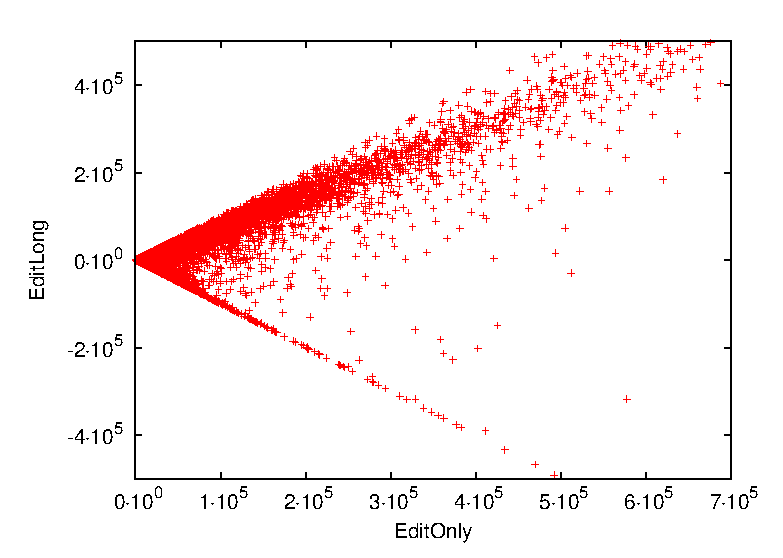
\includegraphics[width=0.45\textwidth]{paper-contrib/score-zoom-editonly-editlong}
    \end{center}
    \caption[EditOnly vs EditLong]{
    	Comparing the absolute edit contribution of a user
	with the edit longevity.
	Notice that authors who are ``all bad''
	are easily identifiable -- and sometimes quite prolific.
    }
    \label{fig-zoom-editonly-editlong}
\end{figure}
%
\begin{figure}[tbph]
    \begin{center}
    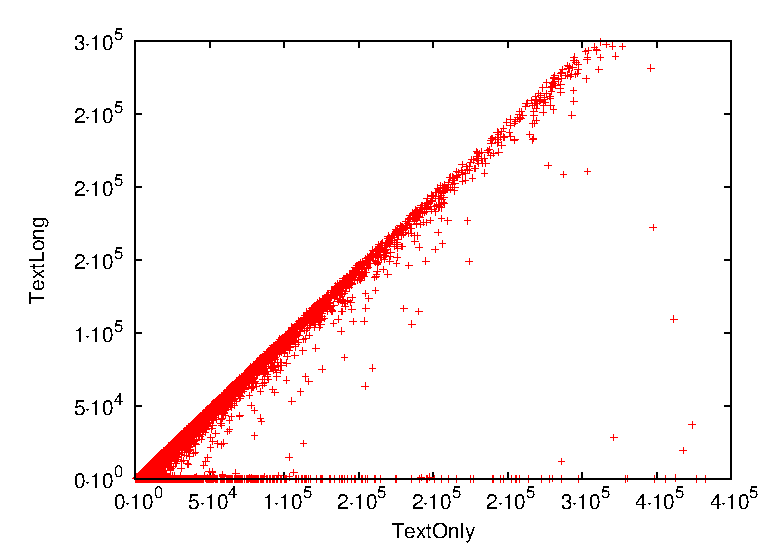
\includegraphics[width=0.45\textwidth]{paper-contrib/score-zoom-textonly-textlong}
    \end{center}
    \caption[TextOnly vs TextLong]{
    	Comparing the absolute text contribution with the contribution
	as measured by text longevity.
	We see that large contributors are either ``all bad''
	or nearly ``all good.''
    }
    \label{fig-zoom-textonly-textlong}
\end{figure}
%
%
\begin{figure}[tbph]
    \begin{center}
    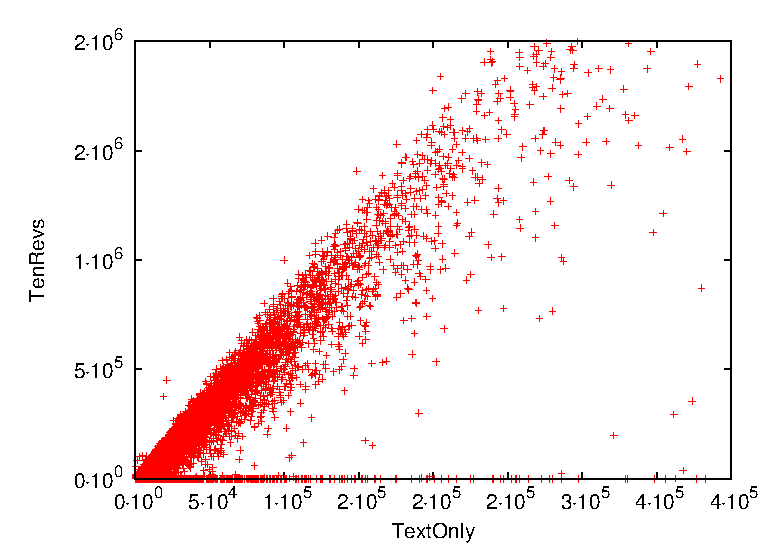
\includegraphics[width=0.45\textwidth]{paper-contrib/score-zoom-revisions-textonly}
    \end{center}
    \caption[Measuring short term text survival]{
    	This graph compares how much text is initially added
	by a user (along the $x$-axis), with how much
	of the text survives over the next ten filtered revisions
	(along the $y$-axis).
	The higher up the $y$-axis a point is, the more
	text that survived all ten revisions.
	Most authors add under 100,000 words,
	and about half of what they add survives.
    }
    \label{fig-zoom-revisions-textonly}
\end{figure}
